\newcommand{\QpuDocTitle}{QPU Getting Started}
\newcommand{\QpuDocSubtitle}{Programming and Website Walkthrough}
\newcommand{\QpuHeaderTitle}{Getting Started}
\newcommand{\QpuDocDescription}{%
A beginner-first introduction to the QPU website, programming vocabulary,
classical logic, complete runnable protocols, and the first steps for correcting
an error.
}
\documentclass[10pt,letterpaper]{article}

% Stable output supports docs:check even when translation uses a temporary directory.
\ifdefined\pdftrailerid
  \pdftrailerid{}
\fi

\usepackage[T1]{fontenc}
\usepackage[utf8]{inputenc}
\usepackage{lmodern}
\usepackage[margin=0.72in]{geometry}
\usepackage{amsmath,amssymb,mathtools}
\usepackage{booktabs,longtable,tabularx,array}
\usepackage[dvipsnames,table]{xcolor}
\usepackage{listings}
\usepackage{tikz}
\usepackage{enumitem}
\usepackage{fancyhdr}
\usepackage{microtype}
\usepackage[hidelinks]{hyperref}
\usepackage{bookmark}
\usepackage{titlesec}

\usetikzlibrary{arrows.meta,calc,positioning}

\definecolor{QpuNavy}{HTML}{0F172A}
\definecolor{QpuBlue}{HTML}{2563EB}
\definecolor{QpuCyan}{HTML}{0891B2}
\definecolor{QpuGreen}{HTML}{047857}
\definecolor{QpuAmber}{HTML}{B45309}
\definecolor{QpuRed}{HTML}{B91C1C}
\definecolor{QpuPaper}{HTML}{F8FAFC}
\definecolor{QpuLine}{HTML}{CBD5E1}
\definecolor{CodeBg}{HTML}{F1F5F9}
\definecolor{CodeComment}{HTML}{64748B}

\providecommand{\QpuDocTitle}{QPU Documentation}
\providecommand{\QpuDocSubtitle}{System Guide}
\providecommand{\QpuDocDescription}{A guide to the QPU circuit system.}
\providecommand{\QpuHeaderTitle}{QPU Documentation}

\hypersetup{
  pdftitle={\QpuDocTitle: \QpuDocSubtitle},
  pdfauthor={Bailey Forbes},
  pdfsubject={QPU protocol syntax, quantum gates, mathematics, and truth tables},
  pdfkeywords={QPU, quantum circuit, protocol, system syntax, truth table}
}

\pagestyle{fancy}
\fancyhf{}
\lhead{\textcolor{QpuNavy}{QPU Circuit Compiler}}
\rhead{\textcolor{QpuNavy}{\QpuHeaderTitle}}
\cfoot{\thepage}
\renewcommand{\headrulewidth}{0.3pt}

\titleformat{\section}{\Large\bfseries\color{QpuNavy}}{\thesection}{0.55em}{}
\titleformat{\subsection}{\large\bfseries\color{QpuBlue}}{\thesubsection}{0.5em}{}
\titleformat{\subsubsection}{\normalsize\bfseries\color{QpuCyan}}{\thesubsubsection}{0.45em}{}
\setlist{nosep,leftmargin=1.5em}
\setlength{\parindent}{0pt}
\setlength{\parskip}{4pt}
\setlength{\tabcolsep}{4pt}
\renewcommand{\arraystretch}{1.15}

\lstdefinelanguage{QPU}{
  morekeywords={
    PARAMS,MAIN-PROCESS,INCREASECYCLE,COMPILEPROCESS,FREE,SET,JOIN,SPLIT,
    CALL,DECLARECHILD,RUNCHILD,REC,TREC,RECUR,EXIT,IF,ELSE,ENDIF,RETURNVALS,ACCEPTVALS,MASTERVAL,SAVE_STATE,
    LOAD_STATE,CREATETOKEN,DELETETOKEN,X,Y,Z,H,S,T,CNOT,CCNOT,CZ,CY,
    SWAP,PHASE,RX,RY,RZ,CPHASE,MEASURE,NOT,AND,NAND,OR,XOR
  },
  sensitive=false,
  morecomment=[l]{\#},
  morecomment=[s]{/*}{*/},
  morestring=[b]"
}
\lstset{
  language=QPU,
  basicstyle=\ttfamily\small,
  keywordstyle=\bfseries\color{QpuBlue},
  commentstyle=\itshape\color{CodeComment},
  backgroundcolor=\color{CodeBg},
  frame=single,
  rulecolor=\color{QpuLine},
  framerule=0.4pt,
  xleftmargin=0.4em,
  framexleftmargin=0.35em,
  columns=fullflexible,
  keepspaces=true,
  showstringspaces=false,
  breaklines=true,
  aboveskip=5pt,
  belowskip=5pt
}

\newcommand{\code}[1]{\texttt{\detokenize{#1}}}
\newcommand{\ket}[1]{\lvert #1\rangle}
\newcommand{\bra}[1]{\langle #1\rvert}
\newcommand{\status}[1]{\textsf{\small #1}}
\newcommand{\implemented}{\textcolor{QpuGreen}{\status{lowered/executed}}}
\newcommand{\acceptedonly}{\textcolor{QpuAmber}{\status{accepted, not executed}}}
\newcommand{\internal}{\textcolor{QpuCyan}{\status{compiler-internal}}}

\newcommand{\GateSegment}[1]{%
\begin{tikzpicture}[baseline=-0.55ex,scale=.78]
  \draw[thick] (0,0)--(3.6,0);
  \node[left] at (0,0) {$\ket{q}$};
  \node[draw=QpuBlue,fill=QpuBlue!8,minimum width=.62cm,minimum height=.55cm,font=\bfseries] at (1.8,0) {#1};
\end{tikzpicture}}

\newcommand{\ControlledSegment}[1]{%
\begin{tikzpicture}[baseline=-0.55ex,scale=.78]
  \draw[thick] (0,.55)--(3.6,.55);
  \draw[thick] (0,-.55)--(3.6,-.55);
  \node[left] at (0,.55) {$\ket{c}$};
  \node[left] at (0,-.55) {$\ket{t}$};
  \fill[QpuNavy] (1.8,.55) circle (.09);
  \draw[thick] (1.8,.55)--(1.8,-.55);
  \node[draw=QpuBlue,fill=QpuBlue!8,circle,inner sep=1.7pt,font=\scriptsize\bfseries] at (1.8,-.55) {#1};
\end{tikzpicture}}

\newcommand{\DoubleControlledSegment}{%
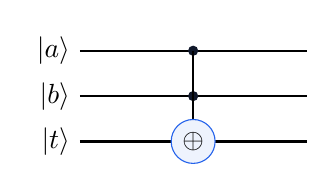
\begin{tikzpicture}[baseline=-0.55ex,scale=.72]
  \foreach \y/\n in {.8/a,0/b,-.8/t} {
    \draw[thick] (0,\y)--(4,\y);
    \node[left] at (0,\y) {$\ket{\n}$};
  }
  \fill[QpuNavy] (2,.8) circle (.09);
  \fill[QpuNavy] (2,0) circle (.09);
  \draw[thick] (2,.8)--(2,-.8);
  \node[draw=QpuBlue,fill=QpuBlue!8,circle,inner sep=2pt,font=\bfseries] at (2,-.8) {$\oplus$};
\end{tikzpicture}}

\newcommand{\SwapSegment}{%
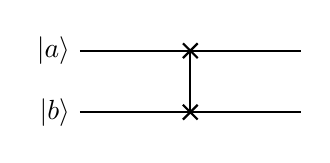
\begin{tikzpicture}[baseline=-0.55ex,scale=.78]
  \draw[thick] (0,.5)--(3.6,.5);
  \draw[thick] (0,-.5)--(3.6,-.5);
  \node[left] at (0,.5) {$\ket{a}$};
  \node[left] at (0,-.5) {$\ket{b}$};
  \draw[thick] (1.68,.38)--(1.92,.62) (1.68,.62)--(1.92,.38);
  \draw[thick] (1.68,-.38)--(1.92,-.62) (1.68,-.62)--(1.92,-.38);
  \draw[thick] (1.8,.5)--(1.8,-.5);
\end{tikzpicture}}

\newcommand{\QpuMeter}[2]{%
  \begin{scope}[shift={(#1,#2)}]
    \draw[QpuBlue,thick] (-0.28,-0.22) rectangle (0.28,0.28);
    \draw[QpuBlue,thick] (-0.18,-0.02) arc (180:0:0.18);
    \draw[QpuBlue,thick] (0,-0.02) -- (0.14,0.16);
    \fill[QpuBlue] (0,-0.02) circle (0.035);
  \end{scope}}
\newcommand{\MeasureSegment}{%
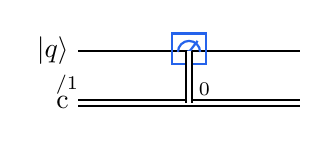
\begin{tikzpicture}[baseline=-0.55ex,scale=.78]
  \draw[thick] (0,0)--(3.6,0);
  \node[left] at (0,0) {$\ket{q}$};
  \QpuMeter{1.8}{0}
  \draw[double distance=1.4pt,thick] (0,-.85)--(3.6,-.85);
  \node[left] at (0,-.85) {c};
  \node[left,font=\scriptsize] at (0.15,-.55) {/1};
  \draw[double distance=1.4pt,thick] (1.8,0)--(1.8,-.85);
  \node[right,font=\scriptsize] at (1.8,-.62) {0};
\end{tikzpicture}}

% The hypertarget gives each gate a stable PDF named destination (gate-CNOT,
% gate-H, ...) that the workbench links to with #nameddest=.
\newcommand{\GateHeading}[3]{%
\subsection{#1 (\code{#2})}\hypertarget{gate-#2}{}
\begin{center}#3\end{center}}

% Short framed callouts. The body is boxed, so it cannot contain lstlisting
% and should stay short enough to fit on one page.
\newsavebox{\QpuCalloutBox}
\newenvironment{QpuCallout}[2]{%
  \def\QpuCalloutColor{#1}%
  \setlength{\fboxrule}{0.6pt}%
  \par\smallskip\noindent
  \begin{lrbox}{\QpuCalloutBox}%
  \begin{minipage}{\dimexpr\linewidth-2\fboxsep-2\fboxrule\relax}%
  \setlength{\parskip}{3pt}%
  {\bfseries\color{#1}#2}\par
}{%
  \end{minipage}%
  \end{lrbox}%
  \fcolorbox{\QpuCalloutColor}{\QpuCalloutColor!6}{\usebox{\QpuCalloutBox}}%
  \par\smallskip
}
\newenvironment{beginnerbox}[1][Beginner note]{\begin{QpuCallout}{QpuGreen}{#1}}{\end{QpuCallout}}
\newenvironment{trybox}[1][Try it in the Circuit builder]{\begin{QpuCallout}{QpuBlue}{#1}}{\end{QpuCallout}}
\newenvironment{cautionbox}[1][Watch out]{\begin{QpuCallout}{QpuAmber}{#1}}{\end{QpuCallout}}

% Workbench selectors on the left, the circuit diagram they produce on the
% right. #1 is the gate name shown in the Gate selector and on the target.
\newcommand{\WorkbenchControlMap}[1]{%
\begin{tikzpicture}[font=\small,>={Latex[length=2mm]}]
  \tikzset{ui/.style={draw=##1,rounded corners=2pt,anchor=west,minimum width=3.9cm,minimum height=.55cm,inner sep=3pt}}
  \node[ui=QpuLine,fill=CodeBg] at (0,1.75) {\textsf{Gate:} \textbf{#1}};
  \node[ui=QpuBlue,fill=QpuBlue!8] (a) at (0,.95) {\textsf{Control A:} \textbf{q0}};
  \node[ui=QpuBlue,fill=QpuBlue!8] (b) at (0,.15) {\textsf{Control B:} \textbf{q1}};
  \node[ui=QpuRed,fill=QpuRed!6] (t) at (0,-.65) {\textsf{Target particle:} \textbf{q2}};
  \node[font=\scriptsize\bfseries,color=QpuNavy,anchor=west] at (0,2.45) {Interactive workbench};
  \node[font=\scriptsize\bfseries,color=QpuNavy] at (7.4,2.45) {Circuit canvas};
  \foreach \y/\q in {.95/q0,.15/q1,-.65/q2} {
    \draw[thick] (5.6,\y)--(9.2,\y);
    \node[left,font=\scriptsize] at (5.6,\y) {\q};
  }
  \draw[->,dashed,QpuBlue] (a.east)--(5.05,.95);
  \draw[->,dashed,QpuBlue] (b.east)--(5.05,.15);
  \draw[->,dashed,QpuRed] (t.east)--(5.05,-.65);
  \fill[QpuNavy] (7.4,.95) circle (.09);
  \fill[QpuNavy] (7.4,.15) circle (.09);
  \draw[thick] (7.4,.95)--(7.4,-.65);
  \node[draw=QpuRed,fill=QpuRed!6,circle,inner sep=1.5pt,font=\bfseries] at (7.4,-.65) {$\oplus$};
  \node[anchor=west,font=\scriptsize] at (9.3,.95) {$A$: read, left unchanged};
  \node[anchor=west,font=\scriptsize] at (9.3,.15) {$B$: read, left unchanged};
  \node[anchor=west,font=\scriptsize] at (9.3,-.65) {$t' = t\oplus(A\land B)$: written};
\end{tikzpicture}}

\newcommand{\QpuTitlePage}{%
\begin{titlepage}
\pagecolor{QpuPaper}
\centering
\vspace*{1.15in}
{\Huge\bfseries\color{QpuNavy} \QpuDocTitle\par}
\vspace{0.2in}
{\LARGE\color{QpuBlue} \QpuDocSubtitle\par}
\vspace{0.55in}
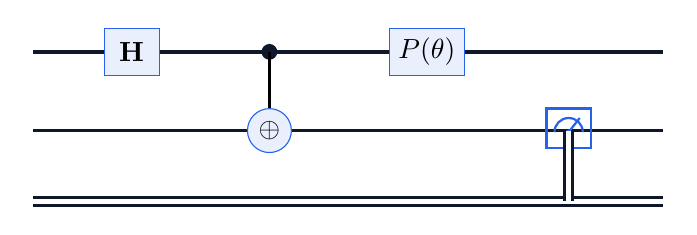
\begin{tikzpicture}
  \draw[very thick,QpuNavy] (0,1)--(8,1);
  \draw[very thick,QpuNavy] (0,0)--(8,0);
  \draw[double distance=1.6pt,very thick,QpuNavy] (0,-.9)--(8,-.9);
  \node[draw=QpuBlue,fill=QpuBlue!10,minimum width=.7cm,minimum height=.6cm,font=\bfseries] at (1.25,1) {H};
  \fill[QpuNavy] (3,1) circle (.1);
  \draw[very thick] (3,1)--(3,0);
  \node[draw=QpuBlue,fill=QpuBlue!10,circle,inner sep=2pt] at (3,0) {$\oplus$};
  \node[draw=QpuBlue,fill=QpuBlue!10,minimum width=.8cm,minimum height=.6cm,font=\bfseries] at (5,1) {$P(\theta)$};
  \QpuMeter{6.8}{0}
  \draw[double distance=1.6pt,very thick,QpuNavy] (6.8,0)--(6.8,-.9);
\end{tikzpicture}
\vfill
{\large Bailey Forbes\par}
{\large September 13, 2026\par}
\vspace{0.35in}
\begin{minipage}{0.82\textwidth}
\small\color{QpuNavy}
\QpuDocDescription
\end{minipage}
\vfill
\end{titlepage}
\nopagecolor
}

% Widen the TOC number column so two-digit subsections (13.10) keep a gap before the title.
\makeatletter
\renewcommand*\l@subsection{\@dottedtocline{2}{1.5em}{2.8em}}
\renewcommand*\l@subsubsection{\@dottedtocline{3}{4.3em}{3.6em}}
\makeatother

\newcommand{\QpuContents}{%
\pagenumbering{roman}
\tableofcontents
\clearpage
\pagenumbering{arabic}
}


\begin{document}
\QpuTitlePage
\QpuContents

\section{How to use the QPU website}

This chapter assumes no programming experience. You can build circuits by
clicking controls, or edit the text protocol directly. Both paths describe the
same circuit.

\subsection{Five programming words used in this guide}

\begin{description}
  \item[Source text] The human-readable instructions in the protocol editor.
  It is ordinary text, like a note, with one QPU instruction per logical line.
  \item[Instruction] One action for the QPU system, such as SET, H, CNOT, or
  MEASURE. The first word says what action to perform.
  \item[Argument] Extra information after an instruction. In
  \code{SET Q 0p}, Q and 0p are arguments: they say which wire and which state.
  \item[Compile] Translate source text into the ordered visual gates that the
  simulator can run. Compilation checks spelling, required inputs, and targets.
  \item[Run] Apply the compiled gates to the selected starting state. Running
  changes simulator state; it does not rewrite the source text.
\end{description}

\subsection{Interface words and how they relate}

\begin{center}
\begin{tabularx}{\textwidth}{>{\bfseries}l X}
\toprule
Word on screen or in source & Meaning\\
\midrule
Particle / qubit & One simulated quantum two-state system. The interface may
say particle where circuit theory says qubit.\\
Wire & The horizontal visual path followed by one qubit through the circuit.\\
Token & A source-text name, such as Q or Carry, that resolves to a wire.\\
Register & One or more qubit wires considered as a group.\\
Gate & A box or controlled symbol that transforms state.\\
Target & The wire changed by a gate.\\
Control & A wire whose state decides whether a controlled gate acts.\\
Protocol / process & The complete source description of a named circuit.\\
\bottomrule
\end{tabularx}
\end{center}

\subsection{Run a bundled example without writing code}

\begin{enumerate}
  \item Open the navigation menu and choose \textbf{Circuit builder}.
  \item Find \textbf{Load a starter circuit} and choose an example.
  \item Inspect the horizontal wires and gate blocks on the circuit canvas.
  \item Choose \textbf{Play Sequence} to watch gates advance, or
  \textbf{Run all} to jump to the final state.
  \item Choose \textbf{Measure all} if the circuit has not already measured
  its outputs.
  \item Read the particle/state display and runtime log. A measured qubit is a
  classical 0 or 1 outcome for that run.
  \item Choose \textbf{Reset state} before repeating the same experiment.
\end{enumerate}

\subsection{Compile a complete protocol}

Listings marked \textbf{Complete runnable protocol} may be copied as a whole:

\textbf{Complete runnable protocol}
\begin{lstlisting}
MAIN-PROCESS FirstWebsiteCircuit
CREATETOKEN -I Q
SET Q 0p
H -I Q -O Q
MEASURE -I Q
RETURNVALS Q
\end{lstlisting}

\begin{enumerate}
  \item Scroll to \textbf{Compile text into a circuit}.
  \item Replace the editor contents with the complete listing.
  \item Choose \textbf{Compile protocol}.
  \item Read \textbf{Protocol checks}. Zero errors means compilation may
  proceed. Warnings identify accepted syntax that may not behave as expected.
  \item Return to the run controls and choose \textbf{Run all}.
\end{enumerate}

\textbf{Expected result:} the H gate prepares equal 0 and 1 amplitudes.
MEASURE returns either 0 or 1. Repeating from Reset state should produce both
outcomes over many runs.

\subsection{Complete examples versus fragments}

This documentation uses three listing labels:
\begin{description}
  \item[Complete runnable protocol] Copy the entire block into the protocol
  editor and compile it.
  \item[Instruction fragment] A few lines demonstrating one syntax rule. Add
  them to a complete process rather than compiling the fragment alone.
  \item[Companion metadata] Truth-table text saved separately as
  \code{.qpuio}; do not paste it into the protocol editor.
\end{description}

\subsection{When protocol checks report a problem}

An \textbf{error} blocks successful compilation. A \textbf{warning} means the
text is accepted but may use inactive, incomplete, or surprising behavior.
Each diagnostic gives a line number, the relevant source line when available,
and a suggested correction.

Choose \textbf{Open Correction Lab for guided help} below the diagnostic list
when the correction is not obvious. The Correction Lab can test a protocol,
probe outputs, explain failures, and propose gate-level guidance. It does not
change protected bundled truth tables.

\subsection{Saving and reopening work}

Choose \textbf{Download as .qpucir} to save protocol source. The
\code{-qpucir.txt} option contains the same source for devices that only handle
plain text files. Use the navigation menu's \textbf{Upload files} page to
reopen a protocol, optionally together with its matching \code{.qpuio}
truth-table metadata.

\section{First circuit: from source to result}

The shortest useful learning path is to prepare one qubit, transform it,
measure it, and declare it as an output:

\textbf{Complete runnable protocol}
\begin{lstlisting}
MAIN-PROCESS FirstCircuit
CREATETOKEN -I Q
SET Q 0p
H -I Q -O Q
MEASURE -I Q
RETURNVALS Q
\end{lstlisting}

\subsection{Read the program line by line}

\begin{enumerate}
  \item \code{MAIN-PROCESS FirstCircuit} gives the protocol a name.
  \item \code{CREATETOKEN -I Q} reserves a logical wire named Q.
  \item \code{SET Q 0p} prepares Q in the basis state $\ket0$.
  \item \code{H -I Q -O Q} applies Hadamard to that same wire, producing
  $\ket+=(\ket0+\ket1)/\sqrt2$.
  \item \code{MEASURE -I Q} samples 0 or 1 and collapses the state.
  \item \code{RETURNVALS Q} declares Q as the first public result.
\end{enumerate}

\begin{center}
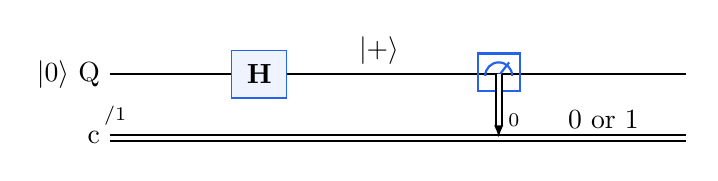
\begin{tikzpicture}[scale=.95]
  \draw[thick] (0,0)--(7.7,0);
  \draw[double distance=1.4pt,thick] (0,-.85)--(7.7,-.85);
  \node[left] at (0,0) {$\ket0$ Q};
  \node[left] at (0,-.85) {c};
  \node[left,font=\scriptsize] at (0.35,-.55) {/1};
  \node[draw=QpuBlue,fill=QpuBlue!8,minimum width=.7cm,minimum height=.6cm,font=\bfseries] at (2,0) {H};
  \node[above] at (3.6,0) {$\ket+$};
  \QpuMeter{5.2}{0}
  \draw[double distance=1.4pt,thick,-{Latex[length=1.6mm]}] (5.2,0)--(5.2,-.85);
  \node[right,font=\scriptsize] at (5.2,-.62) {0};
  \node[above] at (6.6,-.85) {0 or 1};
\end{tikzpicture}
\end{center}

\subsection{What one run means}

One execution gives one random-looking sample. For this circuit, theory predicts
equal probability for 0 and 1. Getting 0 once does not mean H failed, and
getting 1 once does not prove a bias. Repeat the circuit to compare observed
frequencies with the predicted distribution.

\subsection{Adding user-controlled input}

Move a wire into PARAMS when callers or truth-table rows should choose its
start state:

\textbf{Complete runnable protocol}
\begin{lstlisting}
PARAMS: Input:state

MAIN-PROCESS Inverter
X -I Input -O Input
MEASURE -I Input
RETURNVALS Input
\end{lstlisting}
The matching deterministic truth table is:
\begin{center}
\begin{tabular}{c|c}\toprule Input & Output\\\midrule
\code{0p}&\code{1p}\\
\code{1p}&\code{0p}\\\bottomrule
\end{tabular}
\end{center}
The rest of this manual explains every symbol in these examples before moving
to multi-qubit gates, child processes, and full truth-table files.


\section{Classical computation foundations}

Quantum circuits build on ideas from classical digital logic. Understanding
bits, Boolean functions, truth tables, and reversible computation makes the
QPU gate model much easier to use.

\subsection{Classical bits and logical state}

A classical bit has one definite logical value:
\[
b\in\{0,1\}.
\]
Physical computers may represent that value with voltage, charge, magnetic
orientation, or another measurable quantity. Digital logic ignores most
physical detail and works with the abstraction 0 or 1.

A wire carries a bit from one operation to another. A \emph{gate} computes a
function of one or more incoming bits. For example, NOT has one input and one
output:
\[
\operatorname{NOT}(0)=1,\qquad \operatorname{NOT}(1)=0.
\]
In QPU source, a token names the logical wire. On computational-basis states,
\code{X -I Q -O Q} has the same measured input/output relationship as
classical NOT.

\subsection{Boolean algebra}

Boolean algebra describes functions whose values are 0 and 1. This guide uses:
\begin{center}
\begin{tabularx}{\textwidth}{>{\bfseries}l c l X}
\toprule
Operation & Symbol & Spoken form & Meaning\\
\midrule
NOT & $\neg A$ & not A & 1 when A is 0; 0 when A is 1.\\
AND & $A\land B$ & A and B & 1 only when both inputs are 1.\\
OR & $A\lor B$ & A or B & 1 when either or both inputs are 1.\\
XOR & $A\oplus B$ & A exclusive-or B & 1 when exactly one input is 1.\\
NAND & $\neg(A\land B)$ & not-and & The complement of AND.\\
\bottomrule
\end{tabularx}
\end{center}

For bits, XOR is addition modulo two:
\[
0\oplus0=0,\quad 0\oplus1=1,\quad
1\oplus0=1,\quad 1\oplus1=0.
\]
There is no carry in modulo-two addition. Ordinary binary addition handles the
carry separately, which is why a half-adder produces both Sum and Carry.

\subsection{Truth tables as complete finite specifications}

A truth table lists a function's output for every possible input pattern. With
$n$ binary inputs there are $2^n$ patterns. AND, OR, XOR, and NAND can be
compared in one table:
\begin{center}
\begin{tabular}{cc|cccc}
\toprule
$A$&$B$&$A\land B$&$A\lor B$&$A\oplus B$&$\neg(A\land B)$\\
\midrule
0&0&0&0&0&1\\
0&1&0&1&1&1\\
1&0&0&1&1&1\\
1&1&1&1&0&0\\
\bottomrule
\end{tabular}
\end{center}
For a deterministic combinational circuit, this table completely specifies
the classical input/output behavior. It does not reveal the circuit's internal
gate arrangement, propagation time, power consumption, or quantum phase.

\subsection{Combinational logic and stored state}

A \emph{combinational} output depends only on current inputs. Adders and the
Boolean gates above are combinational. A \emph{sequential} circuit also depends
on stored state from an earlier step, as in counters and latches.

QPU cycle suffixes can document successive stages, and INCREASECYCLE marks a
workspace boundary, but the compiled circuit is still one ordered gate
sequence. \code{SAVE_STATE} and \code{LOAD_STATE} copy and restore the simulator
state vector. They are not quantum gates. When modeling stateful behavior
inside the unitary circuit, expose previous state as PARAMS and return next
state through RETURNVALS.

\subsection{Why ordinary classical gates can lose information}

A function is reversible only if each output identifies exactly one input.
Classical NOT is reversible: seeing output 1 proves the input was 0. AND is not:
output 0 could have come from 00, 01, or 10.

\[
(A,B)\xrightarrow{\mathrm{AND}}A\land B
\]
maps four input patterns onto only two output values, discarding information.
Quantum evolution through closed-system gates must be unitary and therefore
reversible. A quantum/reversible AND preserves both inputs and mutates another
target:
\[
(A,B,t)\longmapsto(A,B,t\oplus(A\land B)).
\]
Knowing the output triple lets the transformation be run backward to recover
the input triple. This one-to-one property is one of four conditions a
quantum gate must satisfy to be reversible; \emph{Requirements for a
reversible gate}, in the Theory Guide's mathematical foundations chapter,
states all four together.

\begin{beginnerbox}[How to read $t' = t\oplus(A\land B)$]
\begin{itemize}
  \item $A$ and $B$ are \textbf{controls}. They are only read. After the gate
  they still hold exactly what they held before, which is why the input can
  always be recovered.
  \item $t$ is the \textbf{target}, the output workspace. It is the only wire
  that changes. The prime in $t'$ means ``$t$ after the gate''.
  \item $\oplus$ means ``flip if''. The target flips when $A\land B$ is 1 and
  stays put otherwise.
  \item Start the target at 0 and it ends holding $A\land B$, the ordinary AND
  answer. Start it at 1 and it ends holding NAND instead.
\end{itemize}
In the Circuit builder, $A$ is \textbf{Control A}, $B$ is
\textbf{Control B}, and $t$ is \textbf{Target particle}.
\end{beginnerbox}

\subsection{Controls, targets, and workspace}

These terms connect classical logic to QPU syntax:
\begin{description}
  \item[Control] A wire whose value decides whether a target operation occurs.
  In \code{CNOT -I A -O T}, A is the control.
  \item[Target] The wire changed by an operation. T is the target in that CNOT.
  \item[Workspace or ancilla] An extra wire introduced to hold an intermediate
  or output while preserving inputs. It is commonly initialized to $\ket0$.
  \item[Garbage] Intermediate information left in workspace after the desired
  answer has been computed. Reversible algorithms often \emph{uncompute}
  temporary gates to return garbage wires to zero.
  \item[Uncomputation] Applying inverse operations in reverse order to clean
  workspace without erasing information irreversibly.
\end{description}

The QPU language calls logical wire names tokens. \code{CREATETOKEN} reserves
workspace, SET prepares it, \code{-I} lists inputs/controls, and \code{-O}
names targets.

\subsection{Fan-out, copying, and the no-cloning boundary}

Classical logic freely copies a bit onto several wires. If the source is a
known basis bit and targets begin at zero, CNOT reproduces that basis value:
\[
\ket{x}\ket0\xrightarrow{\mathrm{CNOT}}\ket{x}\ket{x},
\qquad x\in\{0,1\}.
\]
For a superposition $\alpha\ket0+\beta\ket1$, the same circuit produces
\[
\alpha\ket{00}+\beta\ket{11},
\]
not
\[
(\alpha\ket0+\beta\ket1)\otimes
(\alpha\ket0+\beta\ket1).
\]
The first state is generally entangled; the second would be two independent
copies and contains cross terms. The no-cloning theorem forbids a universal
gate that copies every unknown quantum state. QPU aliases similarly give two
names to one wire; they do not create a physical copy.

\subsection{Deterministic, probabilistic, and quantum models}

\begin{tabularx}{\textwidth}{>{\bfseries}p{0.19\textwidth}XXX}
\toprule
Model & State description & Transformation & Observation\\
\midrule
Deterministic classical & One definite bit string & Boolean function &
The definite output bits\\
Probabilistic classical & Probabilities over bit strings & Stochastic update &
A sampled string\\
Pure-state quantum & Complex amplitudes over basis strings & Unitary matrix &
A sampled string after magnitude-squared probabilities and collapse\\
\bottomrule
\end{tabularx}

Negative and imaginary amplitudes are not negative or imaginary probabilities.
They carry phase. Two computational paths can add constructively or cancel
destructively before probabilities are calculated. This interference has no
counterpart in an ordinary classical random-choice table.

\subsection{Classical and QPU operation map}

\begin{center}
\begin{tabularx}{\textwidth}{>{\bfseries}l l X}
\toprule
Classical idea & QPU operation & Important difference\\
\midrule
NOT & X or NOT & Acts linearly on superpositions; X is unitary.\\
XOR into target & CNOT & Preserves the control and can entangle.\\
AND into target & CCNOT or AND & Preserves controls; target is XOR-mutated.\\
Swap variables & SWAP & Exchanges complete quantum wire states.\\
Random bit & H then MEASURE & H first creates coherent amplitudes, not an
ordinary hidden random choice.\\
Read a bit & MEASURE & Sampling collapses a superposition and can disturb
entanglement.\\
Initialize zero & SET token 0p & Compiles to state preparation/reset behavior.\\
Function output & RETURNVALS & Declares an interface; does not itself copy or
measure a wire.\\
\bottomrule
\end{tabularx}
\end{center}


\section{Worked example: reversible half-adder}

A half-adder adds two one-bit numbers without a carry input. Classical theory
defines two outputs:
\[
\mathrm{Sum}=A\oplus B,\qquad
\mathrm{Carry}=A\land B.
\]
The name \emph{half-adder} means it handles half of the full-adder interface:
there is no $C_{\rm in}$ input.

\subsection{Classical specification}

\begin{center}
\begin{tabular}{cc|cc|c}
\toprule
$A$&$B$&Carry&Sum&Binary interpretation\\
\midrule
0&0&0&0&$0+0=00_2$\\
0&1&0&1&$0+1=01_2$\\
1&0&0&1&$1+0=01_2$\\
1&1&1&0&$1+1=10_2$\\
\bottomrule
\end{tabular}
\end{center}
The Carry column is the high-order bit and Sum is the low-order bit. In the
last row, decimal $1+1=2$, written $10_2$ in binary.

\subsection{QPU protocol}

\textbf{Complete runnable protocol}
\begin{lstlisting}
PARAMS: A:state B:state

MAIN-PROCESS HalfAdder
CREATETOKEN -I Carry Sum
SET Carry 0p
SET Sum 0p

XOR -I A B -O Sum
AND -I A B -O Carry

MEASURE -I Carry
MEASURE -I Sum
RETURNVALS Carry Sum
\end{lstlisting}

\subsection{What every term is doing}

\begin{enumerate}
  \item \textbf{PARAMS} declares A and B as caller-controlled state inputs.
  In a basis-state truth-table test they receive \code{0p} or \code{1p}.
  \item \textbf{Carry and Sum are workspace targets.} CREATETOKEN reserves their
  names; SET prepares both in zero.
  \item \textbf{XOR uses A and B as controls/inputs.} It mutates Sum according
  to $s'=s\oplus A\oplus B$. Because $s=0$, the result is $A\oplus B$.
  \item \textbf{AND uses the same preserved controls.} It mutates Carry
  according to $c'=c\oplus(A\land B)$. Because $c=0$, Carry becomes the
  classical carry predicate.
  \item \textbf{MEASURE produces classical samples.} For basis inputs this
  example is deterministic. If A or B is in superposition, outputs may be
  entangled with the inputs and measurement samples a branch.
  \item \textbf{RETURNVALS defines interface order.} Carry is output column
  zero and Sum is output column one. It does not perform measurement itself.
\end{enumerate}

\begin{center}
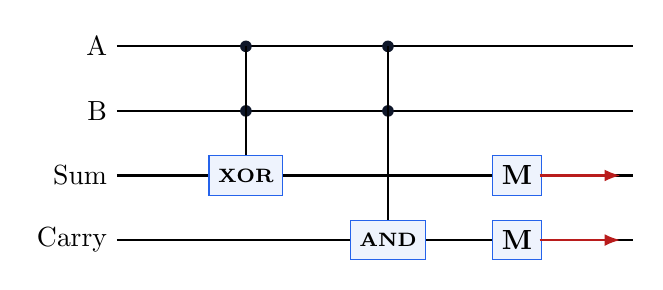
\begin{tikzpicture}[scale=.82]
  \foreach \y/\name in {1.5/A,.5/B,-.5/Sum,-1.5/Carry} {
    \draw[thick] (0,\y)--(8,\y);
    \node[left] at (0,\y) {\name};
  }
  \fill[QpuNavy] (2,1.5) circle (.09);
  \fill[QpuNavy] (2,.5) circle (.09);
  \draw[thick] (2,1.5)--(2,-.5);
  \node[draw=QpuBlue,fill=QpuBlue!8,minimum width=.72cm,minimum height=.5cm,font=\scriptsize\bfseries] at (2,-.5) {XOR};
  \fill[QpuNavy] (4.2,1.5) circle (.09);
  \fill[QpuNavy] (4.2,.5) circle (.09);
  \draw[thick] (4.2,1.5)--(4.2,-1.5);
  \node[draw=QpuBlue,fill=QpuBlue!8,minimum width=.72cm,minimum height=.5cm,font=\scriptsize\bfseries] at (4.2,-1.5) {AND};
  \node[draw=QpuBlue,fill=QpuBlue!8,minimum width=.6cm,minimum height=.5cm,font=\bfseries] at (6.2,-.5) {M};
  \node[draw=QpuBlue,fill=QpuBlue!8,minimum width=.6cm,minimum height=.5cm,font=\bfseries] at (6.2,-1.5) {M};
  \draw[-{Latex[length=2mm]},QpuRed,thick] (6.55,-.5)--(7.8,-.5);
  \draw[-{Latex[length=2mm]},QpuRed,thick] (6.55,-1.5)--(7.8,-1.5);
\end{tikzpicture}
\end{center}

\begin{beginnerbox}[Which wires change?]
Only the two outputs. A and B are \emph{read} by both gates and come out
exactly as they went in. Sum and Carry are \emph{workspace}: they start at 0
and each receives one answer. Keeping the inputs is what makes the circuit
reversible, and it is why a quantum half-adder needs four wires where a
classical one draws two inputs and two outputs.
\end{beginnerbox}

\subsection{Build the Carry gate in the workbench}

The AND line of the protocol corresponds to these workbench choices. With A
on q0, B on q1, and Carry on q2:
\begin{center}
\WorkbenchControlMap{AND}
\end{center}
\begin{trybox}
Choose the \emph{Half adder} starter circuit. Set \textbf{q0 start} and
\textbf{q1 start} to each combination of \code{0p} and \code{1p}, choose
\textbf{Run all} each time, and check the measured Sum and Carry against the
table above.
\end{trybox}

\subsection{Reversible state equation}

Before measurement, the full basis-state action is
\[
\ket{A,B,s,c}\longmapsto
\ket{A,B,s\oplus A\oplus B,\ c\oplus(A\land B)}.
\]
The familiar half-adder is the special case $s=c=0$. Writing the complete
equation avoids a common mistake: XOR and AND do not overwrite arbitrary
targets. They reversibly combine results with the targets' previous states.

\subsection{Companion truth-table metadata}

\begin{lstlisting}
MAIN-PROCESS: HalfAdder
INPUTS: A B
OUTPUTS: Carry Sum
# A B Carry Sum
0 0p 0p 0p 0p
1 0p 1p 0p 1p
2 1p 0p 0p 1p
3 1p 1p 1p 0p
\end{lstlisting}
This file compares the measured QPU outputs with the classical half-adder
specification. Passing all four rows demonstrates basis-state equivalence; it
does not by itself characterize phases for superposition inputs.


\section{Worked example: randomness versus interference}

Classical random choice and quantum superposition can produce identical
single-measurement frequencies. They are not the same theory. This example
uses an intermediate phase change to distinguish them.

\subsection{Classical fair coin model}

Imagine a classical variable R chosen by a fair coin:
\[
P(R=0)=\frac12,\qquad P(R=1)=\frac12.
\]
Once chosen, R is one definite value even if the observer has not looked.
Applying classical NOT changes 0 to 1 and 1 to 0, but the distribution remains
half and half. There is no operation that makes the probability of one hidden
branch cancel the other branch.

\subsection{Quantum preparation with Hadamard}

\begin{lstlisting}
MAIN-PROCESS QuantumCoin
CREATETOKEN -I Q
SET Q 0p
H -I Q -O Q
MEASURE -I Q
RETURNVALS Q
\end{lstlisting}
Before measurement,
\[
\ket0\xrightarrow{H}
\ket+=\frac{\ket0+\ket1}{\sqrt2}.
\]
The amplitudes are $1/\sqrt2$ and $1/\sqrt2$; squaring magnitudes gives the
same half-and-half distribution as the classical coin. If measurement happens
now, this experiment alone cannot distinguish the two descriptions.

\subsection{Insert phase and recombine paths}

\begin{lstlisting}
MAIN-PROCESS PhaseInterference
CREATETOKEN -I Q
SET Q 0p
H -I Q -O Q
Z -I Q -O Q
H -I Q -O Q
MEASURE -I Q
RETURNVALS Q
\end{lstlisting}
Track the state:
\[
\ket0
\xrightarrow{H}
\frac{\ket0+\ket1}{\sqrt2}
\xrightarrow{Z}
\frac{\ket0-\ket1}{\sqrt2}
\xrightarrow{H}
\ket1.
\]

\subsection{Term-by-term explanation}

\begin{description}
  \item[Superposition] After the first H, both basis states have coherent
  amplitudes. No measurement has selected one.
  \item[Phase] Z multiplies only the $\ket1$ amplitude by $-1=e^{i\pi}$. Its
  magnitude remains $1/\sqrt2$, so immediate 0/1 probabilities remain equal.
  \item[Relative phase] The plus relationship between amplitudes becomes a
  minus relationship. A global minus on both terms would not matter; changing
  only one term does.
  \item[Interference] The final H mixes the basis amplitudes. Contributions to
  the $\ket0$ output cancel, while contributions to $\ket1$ add.
  \item[Measurement] The final state is $\ket1$, so measurement returns 1 with
  probability one.
\end{description}

The cancellation can be seen directly from matrix multiplication:
\[
H\frac1{\sqrt2}
\begin{bmatrix}1\\-1\end{bmatrix}
=
\frac12
\begin{bmatrix}1&1\\1&-1\end{bmatrix}
\begin{bmatrix}1\\-1\end{bmatrix}
=
\frac12\begin{bmatrix}0\\2\end{bmatrix}
=\begin{bmatrix}0\\1\end{bmatrix}.
\]
Classical probability weights are nonnegative and would add rather than cancel.
Quantum amplitudes are signed or complex, so phase can create destructive and
constructive interference before the Born rule turns amplitudes into
probabilities.

\subsection{Comparison table}

\begin{center}
\begin{tabularx}{\textwidth}{>{\bfseries}lXX}
\toprule
Question & Classical fair coin & H--Z--H quantum circuit\\
\midrule
State before observation & One hidden definite bit sampled fairly &
Coherent complex amplitude vector\\
Effect of middle sign/phase & No probability analogue that preserves a fair
distribution and later cancels a branch & Z changes relative phase without
changing immediate basis probabilities\\
Can paths cancel? & No; probabilities add & Yes; amplitudes add and may cancel\\
Final result in this example & Still a distribution unless another classical
rule forces a value & Deterministic 1\\
\bottomrule
\end{tabularx}
\end{center}



\section{Where to continue}

\begin{itemize}
  \item Read \textbf{QPU Theory Guide} when amplitude, phase, or matrix notation
  is unfamiliar.
  \item Open \textbf{QPU Language Reference} while writing exact syntax.
  \item Open \textbf{QPU Examples and Troubleshooting} when Protocol checks
  reports an error or a truth-table test fails.
\end{itemize}

\end{document}
